% !TeX spellcheck = en_GB 

\section{\label{sec::results}Results}

In the following we want to show some results of our simulations. If not explicitly mentioned, we used the properties described in section \ref{sec::modelling}.

The first thing we will have a closed look at, is a constant Dirichlet boundary. With this we can model an oven with relatively fast circulating air, so the outermost layer is always covered with hot air. In figure \ref{fig::dirichlet2D} we can see the heating progress of this model. Interesting to notice is, that the aluminium stick is almost completely heated to $200\SI{}{\degreeCelsius}$ after one minute.

\begin{figure}[htp]
	\centering
	\makebox[\textwidth][c]{
	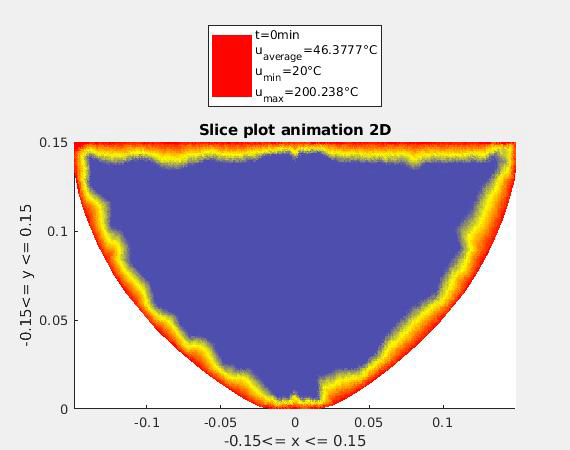
\includegraphics[width=0.69\textwidth]{figures/dirichlet_200_2D001.png}
	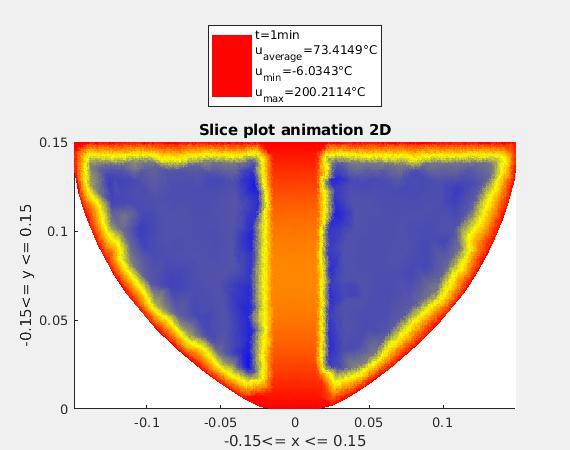
\includegraphics[width=0.69\textwidth]{figures/dirichlet_200_2D002.png}
	}
	\makebox[\textwidth][c]{
	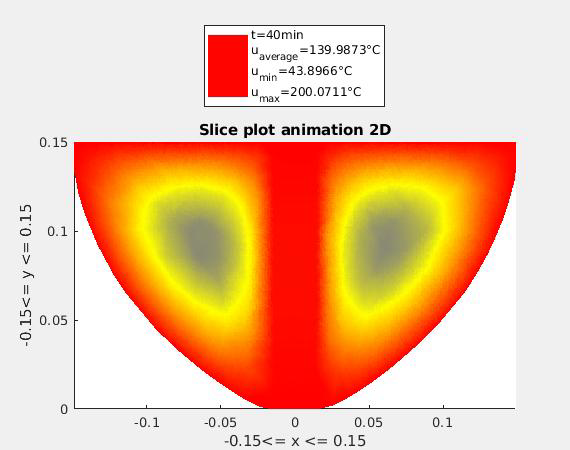
\includegraphics[width=0.69\textwidth]{figures/dirichlet_200_2D041.png}
	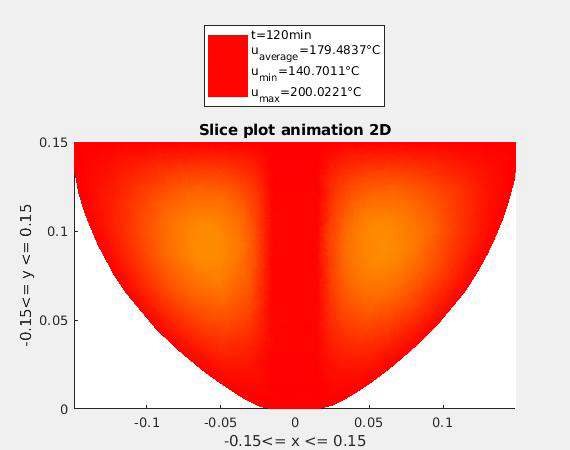
\includegraphics[width=0.69\textwidth]{figures/dirichlet_200_2D121.png}
	}
	\caption{\label{fig::dirichlet2D} side view of 200\SI{}{\degreeCelsius} Dirichlet boundary}
\end{figure}

As people tend to be impatient, it might also be interesting, to consider the case, in which we heat up the oven, while the cake is already in it. This is modelled by time dependent Dirichlet conditions. For the example in figure \ref{fig::dirichletHeat2D} we heated up the oven quite slowly, so the effect can be seen better. Of course the average temperature in this case rises slower. Compared to the constant boundary the average and the minimal temperature stay closer together here. We are not experts in baking, but maybe there are situations, where this is an advantage.

\begin{figure}[htp]
	\centering
	\makebox[\textwidth][c]{
	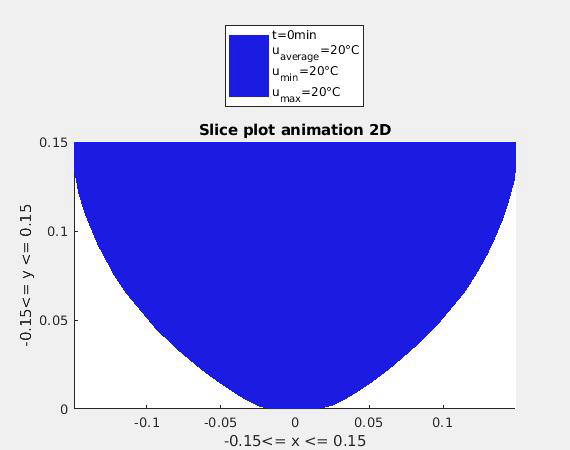
\includegraphics[width=0.69\textwidth]{figures/dirichlet_heat_200_2D001.png}
	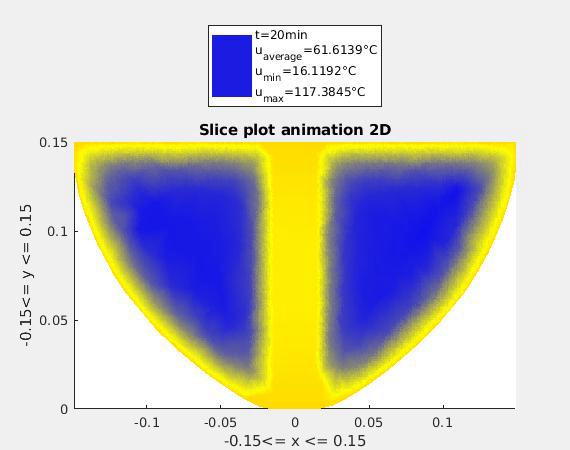
\includegraphics[width=0.69\textwidth]{figures/dirichlet_heat_200_2D021.png}
	}
	\makebox[\textwidth][c]{
	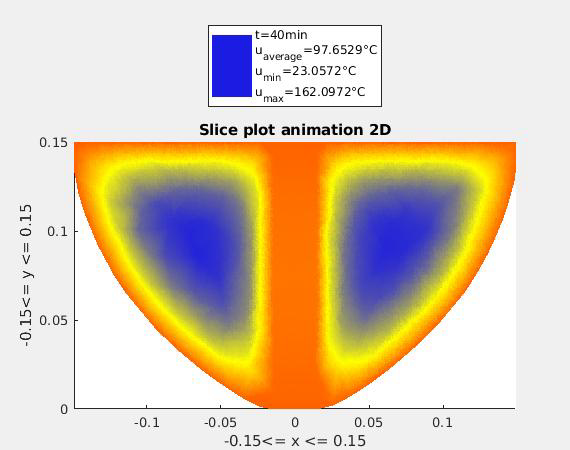
\includegraphics[width=0.69\textwidth]{figures/dirichlet_heat_200_2D041.png}
	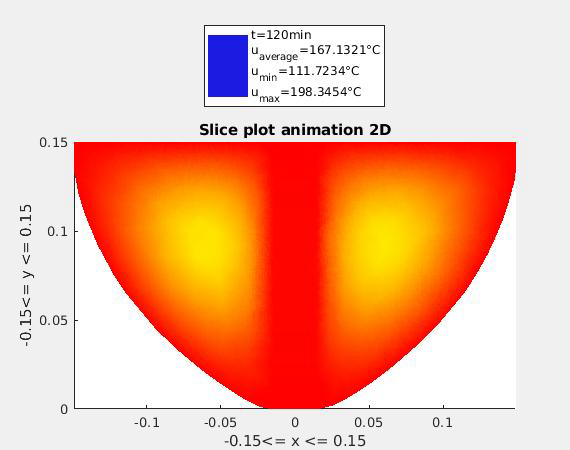
\includegraphics[width=0.69\textwidth]{figures/dirichlet_heat_200_2D121.png}
	}
	\caption{\label{fig::dirichletHeat2D} side view heating Dirichlet boundary boundary}
\end{figure}

In the previous examples we saw, how the aluminium stick in the middle heated up the cake from the inside. To see, how much influence on the baking progress it actually had, we modelled the whole process without the aluminium in figure \textbf{missing plots here}. \textbf{missing obsevation here}.